\documentclass[12pt,a4paper]{article}

\usepackage{tabularx}
\usepackage{geometry}
\usepackage{tikz}
\usepackage{verbatim}
\usepackage{amsmath}
\usepackage[utf8]{inputenc}


\def\mavis{{\itshape MAvis}}

\usepackage{graphicx}
\graphicspath{{figures/}}

\newcommand{\showlevel}[2]{%
    \scalebox{1}[.74]{%
        \begin{minipage}{#2}
            \renewcommand{\baselinestretch}{0.8}
            \verbatiminput{#1.lvl}
            \renewcommand{\baselinestretch}{1.0}
        \end{minipage}
    }
}
%\end{verbatim}%TexMaker is syntax-hightlight-confused by the \verbatiminput command above. The \end{verbatim} unconfuses it from here on (even though it's commented out).

\title{\mavis\ Domain Description: The Hospital Domain}

\author{Thomas Bolander, Mikkel Birkegaard Andersen, Andreas Garn\ae s, \\ Lasse Dissing Hansen, Martin Holm Jensen, Mathias Kaas-Olsen}


\geometry{ 
  includeheadfoot,
  margin=2.3cm
}


\newcommand{\jt}[1]{\texttt{#1}}

\tikzset{%
    agent/.style={circle,fill,minimum size=8mm,inner sep=0pt},
    wall/.style={rectangle,fill,minimum size=10mm,black},
    trans/.style={rectangle,fill,minimum size=7mm},
    unknown/.style={rectangle,fill,minimum size=10mm,gray},
    goal/.style={rectangle,fill,minimum size=9.5mm,yellow},
    ggoal/.style={rectangle,fill,minimum size=9.5mm,green}
}

\newcommand{\textenv}[1]{\color{black}{\textbf{\LARGE #1}}}
\newcommand{\dd}{\draw[step=10mm] (0,0) grid (60mm,40mm); \foreach \i in {5,15,...,35} \node[wall] at (5mm,\i mm) {}; \foreach \i in {5,15,...,65} \node[wall] at (\i mm,5mm) {}; \foreach \i in {5,15,...,55} \node[wall] at (\i mm,35mm) {}; \node[wall] at (65mm,15mm) {}; \node[wall] at (65mm,25mm) {}; \node[wall] at (55mm,25mm) {};}



\begin{document}
    \maketitle

\abstract{This document describes the hospital domain of the \mavis\ visualisation tool.}


\section{Domain background and motivation}
The hospital domain is partly inspired by the developments in mobile robots for hospital use and systems of warehouse robots like the KIVA robots at Amazon, see Figure~\ref{figu:kiva}. In both applications, there is a high number of transportation tasks to be carried out. Among the most successful and widely used implementation of hospital robots so far are the TUG robots by the company Aethon, see Figure~\ref{figu:tug2}. TUG robots were first employed in a hospital in 2004, and is now in use in more than 100 hospitals in the US. Since 2012, TUG robots have also been applied at a Danish hospital, Sygehus Sønderjylland, the first hospital in Europe to employ them. 
\begin{figure}
    \hfill
    \begin{minipage}[b]{.44\textwidth}
\begin{center}
        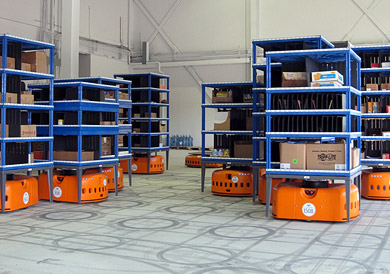
\includegraphics[width=\textwidth]{kiva}
\end{center}
        \caption{KIVA robots at Amazon.}
        \label{figu:kiva}
    \end{minipage}
    \hfill
   \begin{minipage}[b]{.3\textwidth}
   \begin{center}
        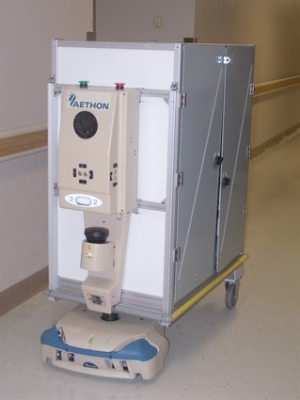
\includegraphics[width=0.7\textwidth]{TUGtugging}
\end{center}
        \caption{The TUG robot tugging a container.}
        \label{figu:tug2}
    \end{minipage}
    \hfill
\end{figure}
The hospital domain of \mavis\ supports a simplified simulation of transportation robots at a hospital or in a warehouse.
  
\section{Levels}\label{sec:env_description}
\begin{figure}
  \begin{center}
    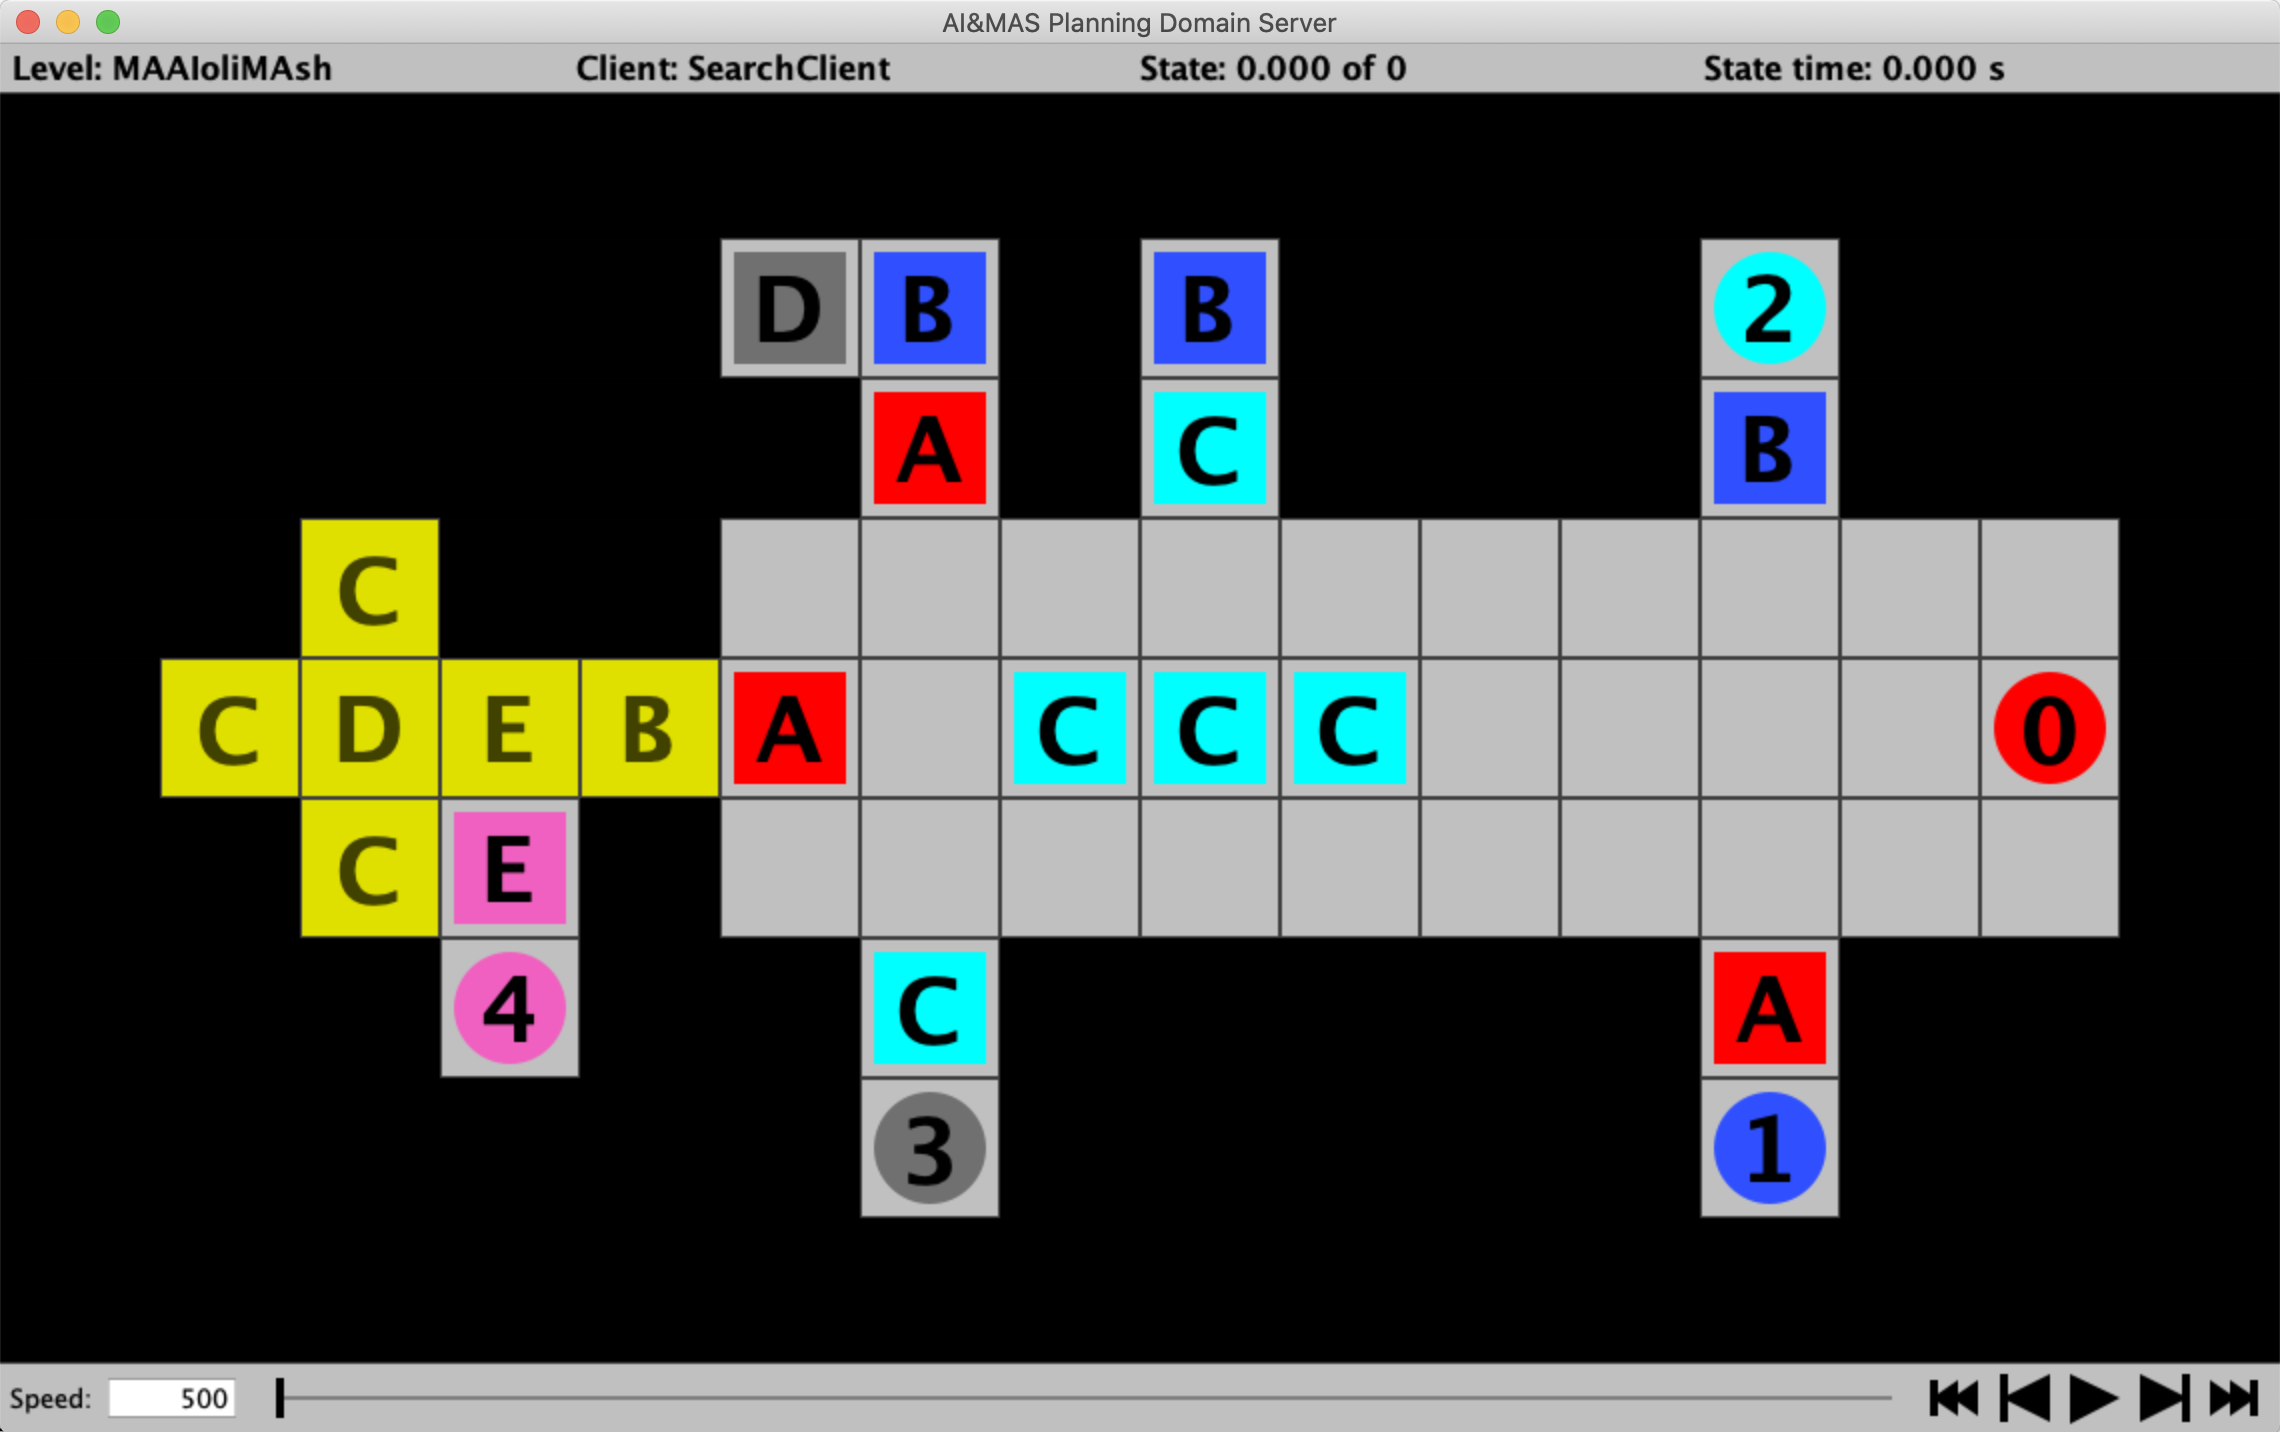
\includegraphics[width=0.65\textwidth]{MAAIoliMAsh}
  \end{center}
  \caption{Example level as visualised in the \mavis\ visualisation environment. }\label{figu:aioli}
\end{figure}
Levels of the hospital domain are grid-based environments. Figure~\ref{figu:aioli} shows the visualisation of an example level. A level in the hospital domain contains \emph{walls}, \emph{boxes}, \emph{goal cells}, and \emph{agents}. The \emph{walls} are used to represent the physical layout of the environment, visualised as black squares. The \emph{agents} represent the robots, visualised as numbered colored circles. The \emph{boxes} represent the items that the robots have to move, visualised as lettered colored squares. The \emph{goal cells} represent destinations, visualised as yellow circles and squares with numbers or letters corresponding to agents or boxes. To \emph{solve} a level, each goal cell must have an object of the correct type on top of it: each yellow square must have a box of the same letter on top of it, and each yellow circle must have the agent with the correct number on top of it. In the level of Figure~\ref{figu:aioli}, only the boxes have destinations.  Agents can only move boxes that have the same color as themselves.  


\begin{figure}
\begin{center}
    \scalebox{1.2}{\showlevel{levels/MAExample}{1.5cm}}
    \hspace{3cm}
    \raisebox{-18mm}{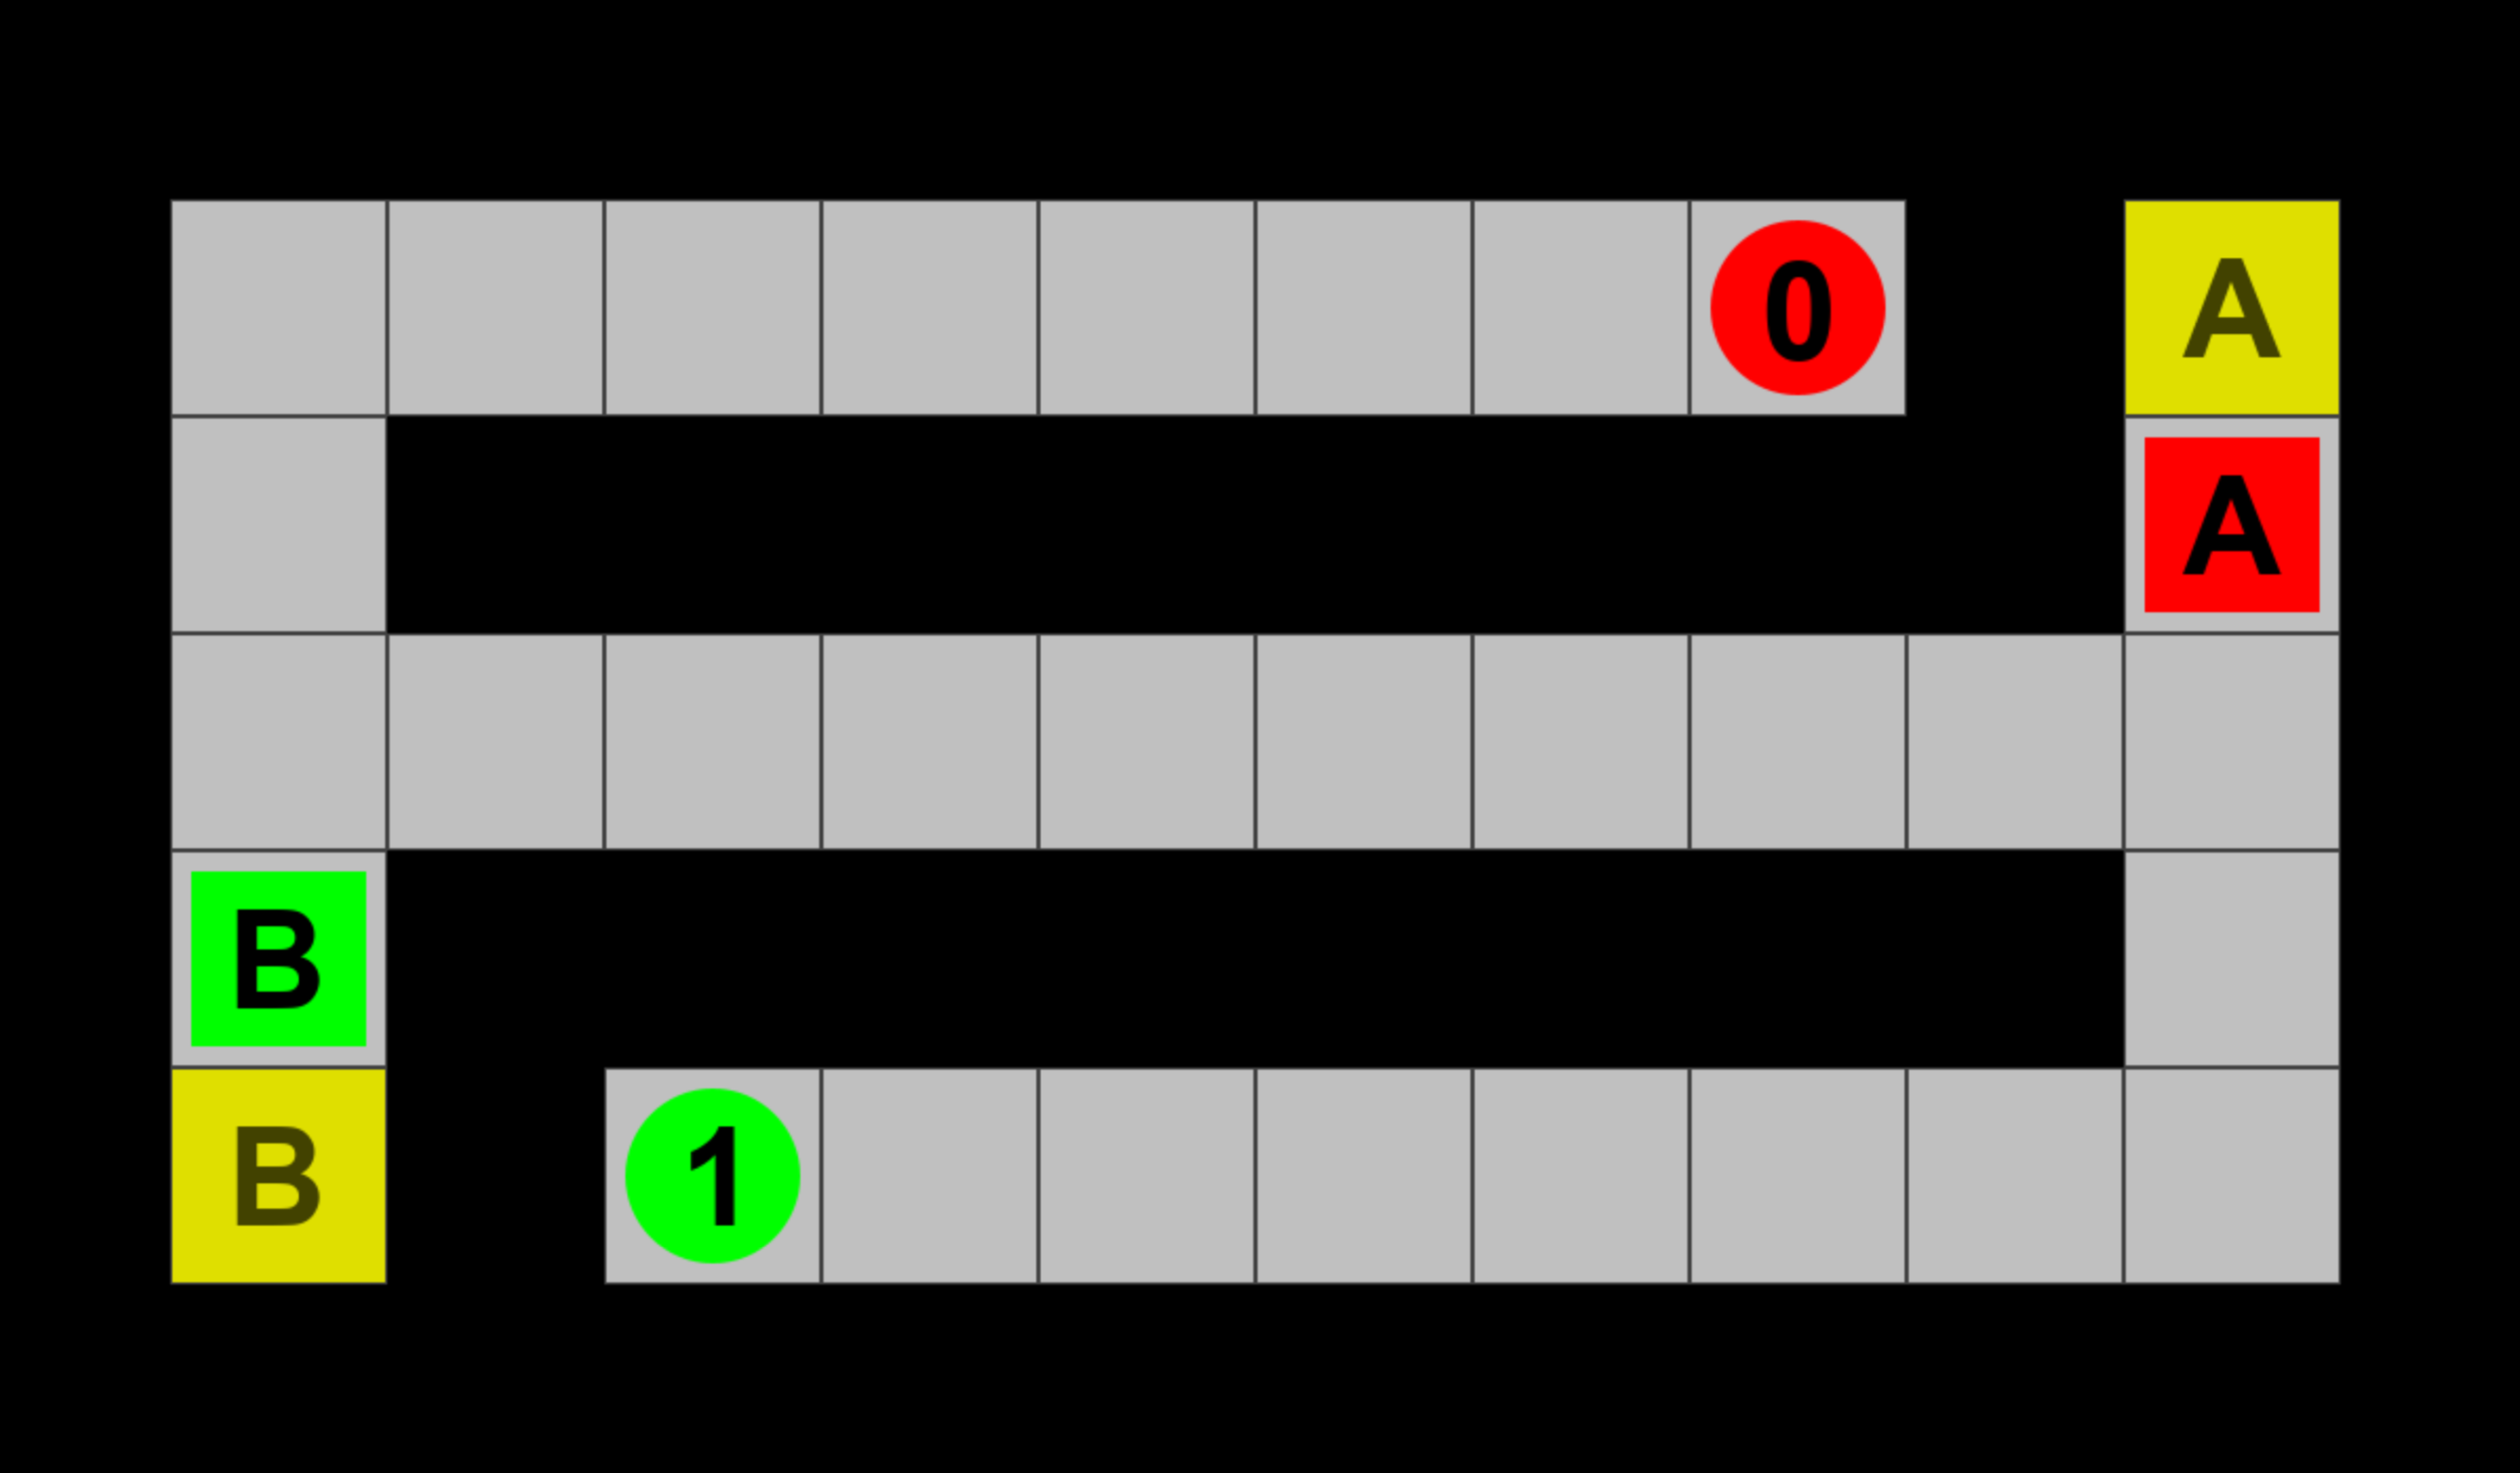
\includegraphics[width=7cm]{MAExample}}
\end{center}
\caption{The textual representation of a level (left), and its graphical visualisation (right).}\label{figu:textual}
\end{figure}
Levels are defined using a textual format, making it easy to design levels using any decent text editor (with a monospaced font) and saving the levels in ASCII-encoded text files. Figure~\ref{figu:textual} shows a full textual description of a simple level (left) accompanied by its graphical visualisation in \mavis\ (right). In this level, agent \texttt{0} can only move box \texttt{A}, and agent \texttt{1} only box \texttt{B}. Below we describe the detailed syntax of the textual representation of levels. 

\subsection{Overall level format} 
\begin{figure}
\begin{center}
\begin{tabular}{l}
\verb|#domain| \\
\verb|hospital| \\
\verb|#levelname| \\
\verb|<name>| \\
\verb|#colors| \\
\verb|<colors>| \\
\verb|#initial| \\
\verb|<initial>| \\
\verb|#goal| \\
\verb|<goal>| \\
\verb|#end| 
\end{tabular}
\end{center}
\caption{The level format of the hospital domain.}\label{figu:level-format}
\end{figure}
Each level file is formatted according to the syntax provided in Figure~\ref{figu:level-format}.
The items in angle brackets (e.g. \texttt{<name>}) are placeholders for content described below, and all lines are terminated by either a line-feed character (LF) or a carriage-return followed by a line-feed (CRLF).
The first two lines indicate the domain of the problem, which in this case is the hospital domain, and occur verbatim in level files. The \texttt{<name>} field is replaced by the level's name.

\subsection{Initial state and goal state}
Levels are constructed with initial and goal states using the following conventions:
\begin{itemize}
    \item \emph{Walls} are represented by the symbol \verb|+|.
    \item \emph{Agents} are represented by the numbers \verb|0,1,...,9|, with each number identifying a unique agent, so there can be at most 10 agents present in any given level. The present agents must be consecutively numbered starting from \verb|0|. For example, a level with two agents must use \verb|0| and \verb|1| and not e.g. \verb|3| and \verb|9|.
    \item \emph{Boxes} are represented by capital letters $\verb|A|, \verb|B|, \dots, \verb|Z|$. The letter is used to denote the \emph{type} of the box, e.g.\ one could use the letter \verb|B| for hospital beds. There can be several boxes of the same type (i.e.\ same letter) in a level.
     \item \emph{Free cells} (i.e.\ any cell that is not a wall, an agent or a box) are represented by spaces (ASCII value 32).
\end{itemize}
The \texttt{<initial>} and \texttt{<goal>} specifications consist of lines with these symbols as a top-down map, which defines the initial state and goal states of the planning problem respectively. The two specifications must have exactly matching configurations of walls, and should consist of at most $2^{15} - 1$ rows each of at most $2^{15} - 1$ columns. It is required that the agent and all boxes in a level are in areas entirely enclosed by walls. Each symbol in the initial state specifies that a corresponding object starts in that position, and each symbol in the goal state specifies that for the level to be solved, an object of the symbol's type must occupy that cell. The goal states of the planning problem are then all states which have objects in the configuration shown in \texttt{<goal>}, where excess objects can be anywhere (i.e.\ the agent and/or some boxes do not necessarily have to have a goal cell they must reach to solve a level).

\subsection{Colors}
To allow modelling of different agents having different abilities concerning which boxes they can and can't move, agents and boxes are given colors. An agent can only move a box that has the same color as itself. If we for example use boxes of type B to represent beds, and if these are red, then only the red agents can move beds.

The \emph{allowed colors} for the agents and boxes are:
\begin{center}
blue, red, cyan, purple, green, orange, pink, grey, lightblue, brown.
\end{center}
To represent the colors of the agents and boxes as part of the textual level representation, each level has the colors section (\texttt{\#colors}). The color declaration \texttt{<colors>} is of the form
\begin{verbatim}
<color>: <object>, <object>, ..., <object>
<color>: <object>, <object>, ..., <object>
...
<color>: <object>, <object>, ..., <object>
\end{verbatim}
where each \texttt{<color>} is an allowed color, and each \texttt{<object>} is either a box type (\texttt{A}, $\dots$, \texttt{Z}) or an agent (\texttt{0}, $\dots$, \texttt{9}). Note that this specification forces all boxes of a type to have the same color, e.g.\ there can't be both a blue and a red \texttt{A} box; all \texttt{A} boxes must have the same color. Each agent and box type used in a level must occur exactly once in the color declaration of the level, and the declaration may not contain objects that are not present in the level.

\section{Actions}\label{sect:actions}
A grid cell in a level is called \emph{occupied} if it contains either a wall, an agent, or a box. A cell is called \emph{free} if it is not occupied. Each agent can execute four different types of actions: \emph{moves}, \emph{pushes}, \emph{pulls} and a \emph{no-op}. 

\subsection{Move}
%\begin{enumerate}
%\paragraph{Move action} 
A move action is represented in the textual form
    \[
        \texttt{Move(<move-dir-agent>)}        
            \]
    where \texttt{<move-dir-agent>} is one of \texttt{N} (north), \texttt{W} (west), \texttt{S} (south), or \texttt{E} (east). \texttt{Move(N)} means to move one cell to the north of the current location. For a move action to be \emph{applicable}, the following must be the case:
    \begin{itemize}
        \item The neighboring cell in direction \texttt{<move-dir-agent>} is currently free.
    \end{itemize}

\subsection{Push} A push action is represented in the textual form
    \[
        \texttt{Push(<move-dir-agent>,<move-dir-box>)}
    \]
    Here \texttt{<move-dir-agent>} is the direction that the agent moves in, as above. The second parameter, \texttt{<move-dir-box>}, is the direction that the box is pushed in. The following example illustrates a push:
    \begin{center}
       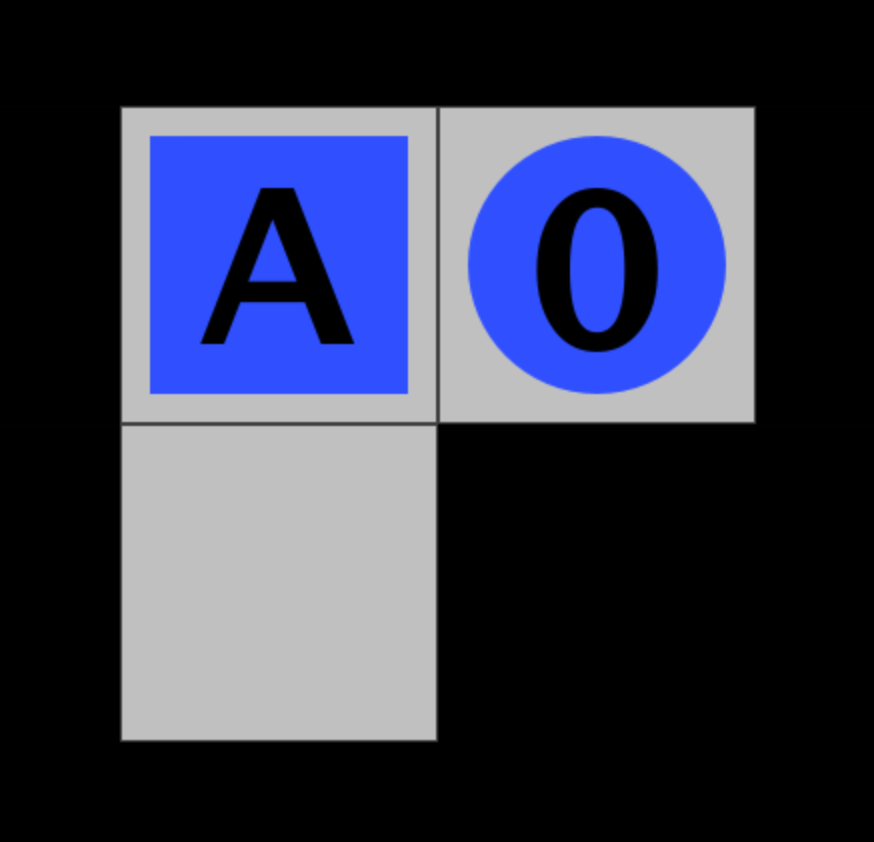
\includegraphics[width=2cm]{action_example1}  \quad
    \raisebox{8mm}{$\xrightarrow{\texttt{Push(W,S)}}$} \quad 
      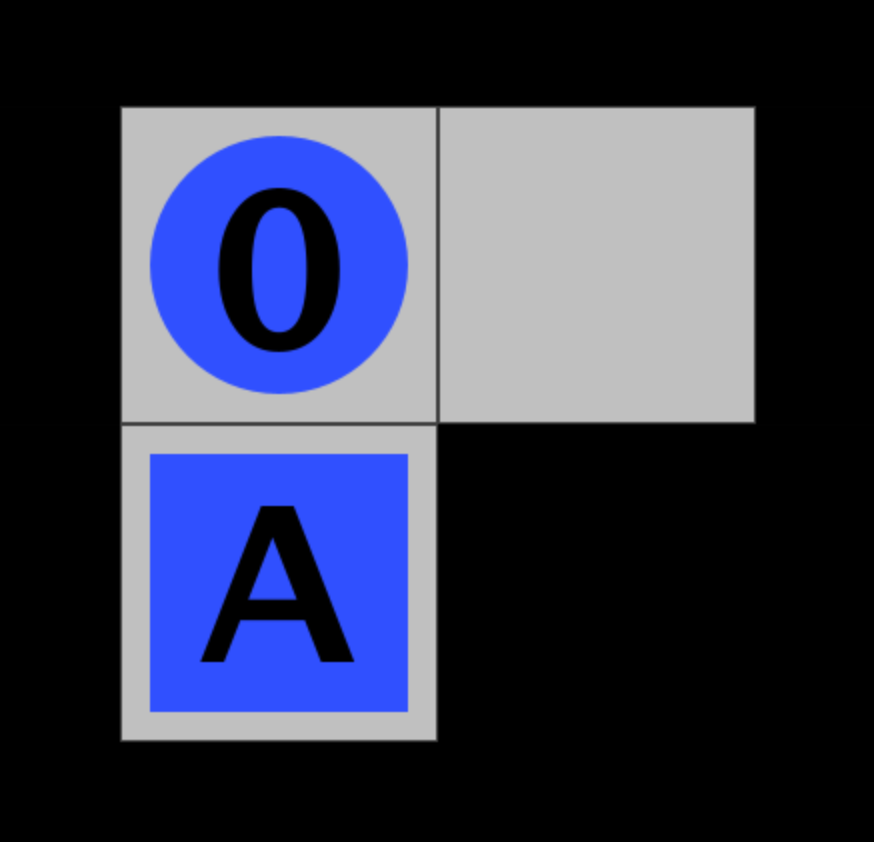
\includegraphics[width=2cm]{action_example2}
    \end{center}
    Here the agent, \verb|0|, moves west and the box, \verb|A|, moves south. The box is ``pushed around the corner.'' For a push action to be \emph{applicable}, the following must be the case:
    \begin{itemize}
        \item The neighbouring cell of the agent in direction \texttt{<move-dir-agent>} contains a box $\beta$ of the same color as the agent.
        \item The neighbouring cell of $\beta$ in direction \texttt{<move-dir-box>} is currently free.
    \end{itemize}
    The result of an applicable push action will be that the agent moves one cell in direction \texttt{<move-dir-agent>}, and that $\beta$ moves one cell in direction \texttt{<move-dir-box>}. Note that the second condition above ensures that it is not possible for the agent and the box to swap positions by simply performing an action like \texttt{Push(W,E)}.

\subsection{Pull} A pull action is represented in the textual form
    \[
        \texttt{Pull(<move-dir-agent>,<move-dir-box>)}
    \]
    Both parameters are as for pushes. The following example illustrates a pull, reversing the push shown above:
    \begin{center}
       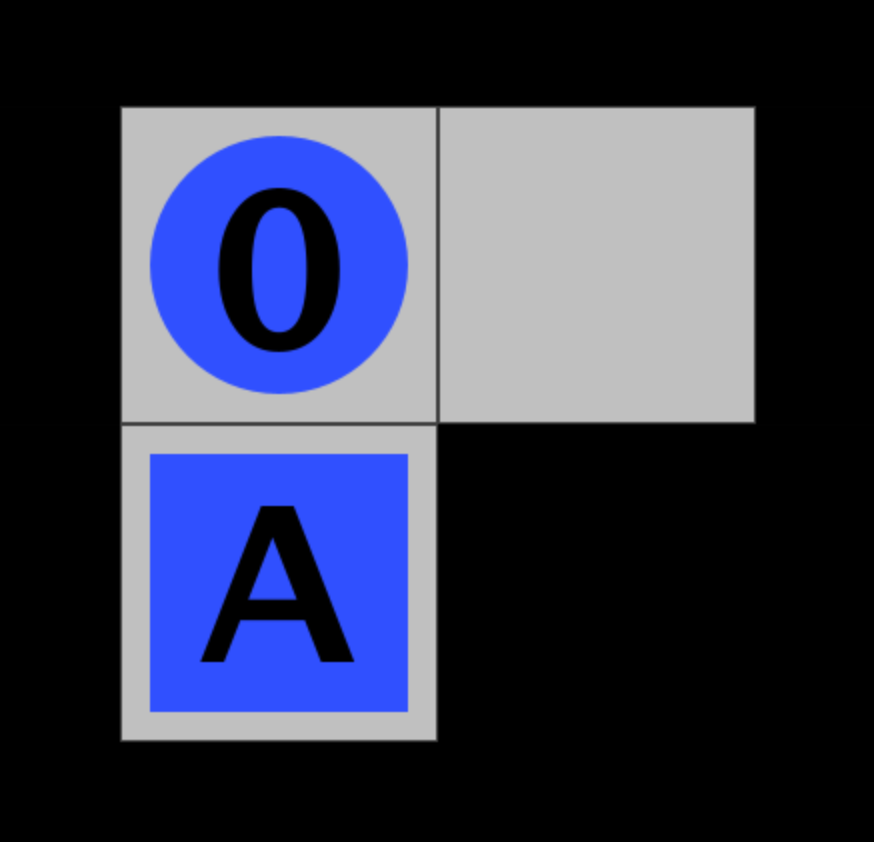
\includegraphics[width=2cm]{action_example2} \quad
        \raisebox{8mm}{$\xrightarrow{\texttt{Pull(E,N)}}$} \quad  
         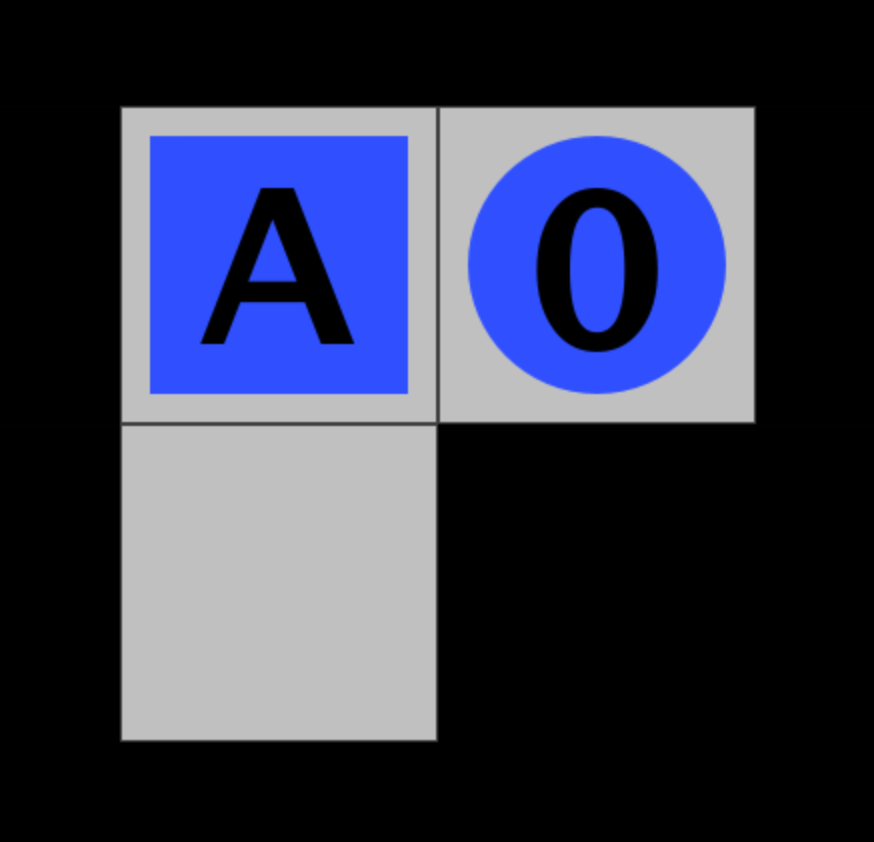
\includegraphics[width=2cm]{action_example1}
    \end{center}
    For a pull action to be \emph{applicable}, the following must be the case:
    \begin{itemize}
        \item The neighbouring cell of the agent in direction \texttt{<move-dir-agent>} is currently free.
        \item The neighbouring cell of the agent in the \emph{opposite} direction of \texttt{<move-dir-box>} contains a box $\beta$ of the same color as the agent (where \texttt{N} and \texttt{S} are opposite directions of each other, and similarly for \texttt{W} and \texttt{E}).
    \end{itemize}
    The result of an applicable pull action will be that the agent moves one cell in direction \texttt{<move-dir-agent>}, and that $\beta$ moves one cell in direction \texttt{<move-dir-box>}. Note that the first condition ensures that a swap is not possible.
   
\subsection{No-op} The no-op (no operation) action is represented in the textual form \texttt{NoOp}. The action represents the agent doing nothing. It has no parameters and is always \emph{applicable}.
%\end{enumerate}

\subsection{Applicability and inapplicability}
The applicability of each individual action is specified above. If an agent tries to execute an inapplicable action, it will fail. Failure corresponds to performing a no-op action, i.e.\ doing nothing. So if an agent e.g.\ tries to move into an occupied cell, it will simply stay in the same cell. 

\subsection{Callouts}
Agents can callout short messages which will be shown in a speech bubble above the agent using the textual representation
\[
  \texttt{<action>@<message>}
\]
where \texttt{<message>} is the optional message string that will be shown in the speech bubble.
This feature can used for visualizing agent intentions or debugging purposes.
Note that the functionality is purely cosmetic and does not affect action execution.

\subsection{Joint actions and conflicts}
If a level has several agents, these agents can perform simultaneous actions. The actions of the individual agents are assumed to be completely synchronised, hence we consider joint actions, which have the textual representation
\[
  \texttt{<action0>|<action1>|...|<action9>}
\]
In a joint action, \texttt{<action0>} is the action performed by agent \texttt{0}, \texttt{<action1>} is the action performed by agent \texttt{1}, etc. Which cells are occupied is always determined at the beginning of a joint action, so it is e.g.\ not possible for one agent to move into a cell in the same joint action as another one leaves it. Simultaneous actions can be \emph{conflicting} if two or more agents try to move either themselves or boxes into the same cell, or if two agents attempt to move the same box. If this happens, then neither agent will succeed in their action, and both agents perform a \texttt{NoOp} instead.

\subsection{Solving a level}

\begin{figure}
\begin{center}
%  \scalebox{1.2}{
  \showlevel{levels/SAsimple0}{1.5cm}
 % }
\end{center}
\caption{A simple level, \texttt{SAsimple0.lvl}.}\label{figu:simple_level}
\end{figure}
\begin{figure}
\begin{center}
  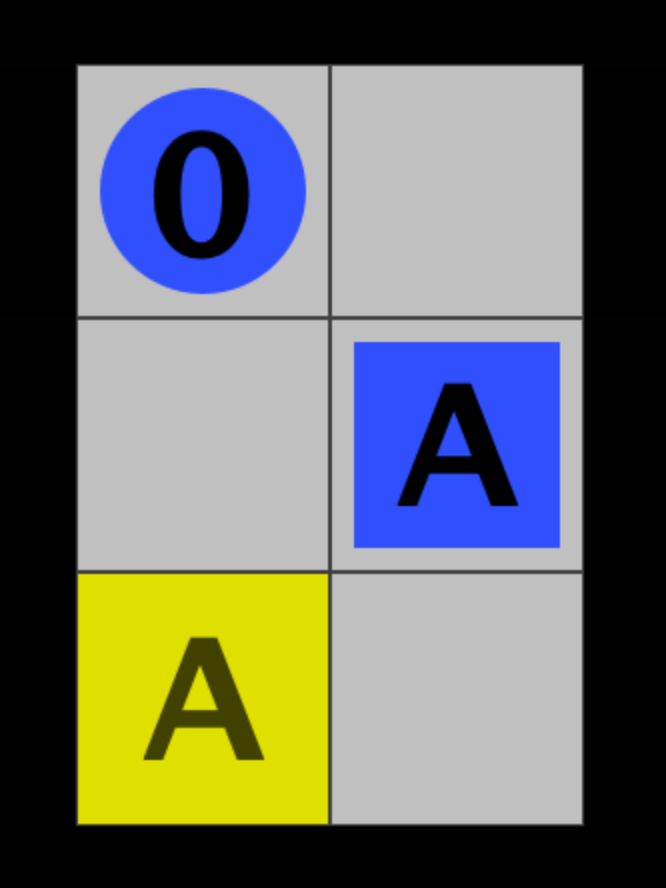
\includegraphics[width=2cm]{simple0_1} 
\quad
        \raisebox{12mm}{$\xrightarrow{\texttt{Move(S)}}$} 
\quad  
  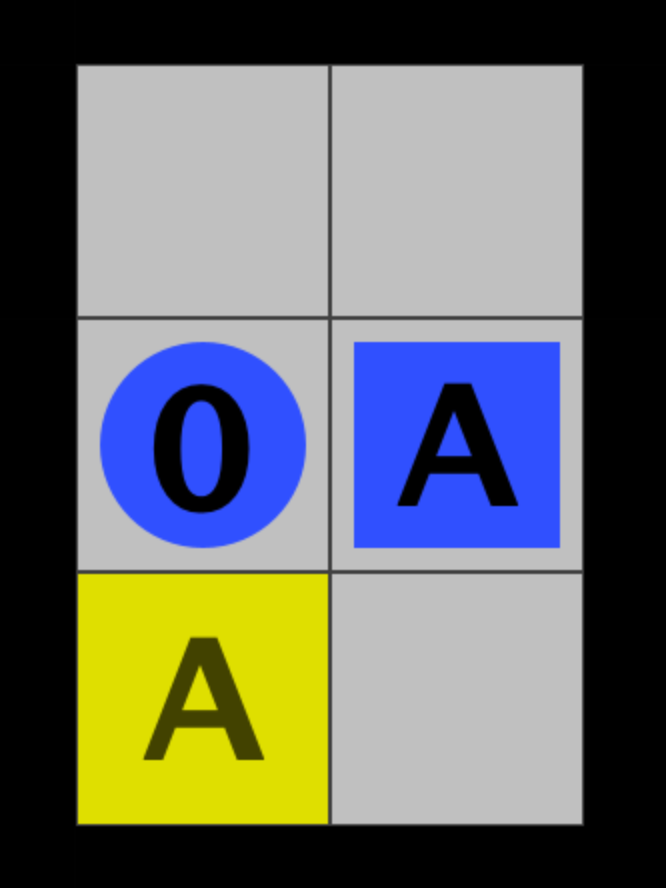
\includegraphics[width=2cm]{simple0_2} 
\quad
 \raisebox{12mm}{$\xrightarrow{\texttt{Pull(N,W)}}$} 
\quad
  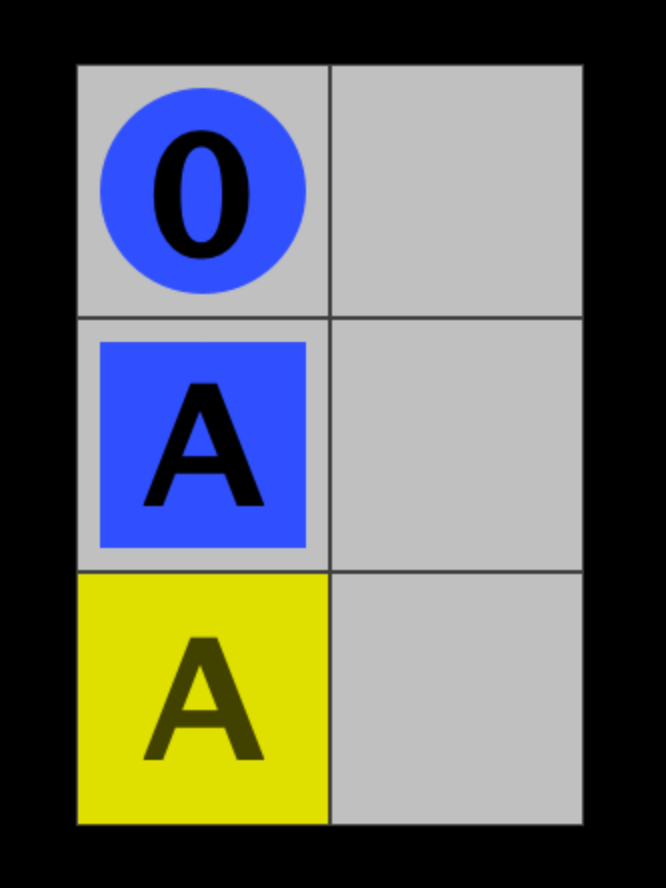
\includegraphics[width=2cm]{simple0_3} 
\quad
 \raisebox{12mm}{$\xrightarrow{\texttt{Push(S,S)}}$} 
\quad
  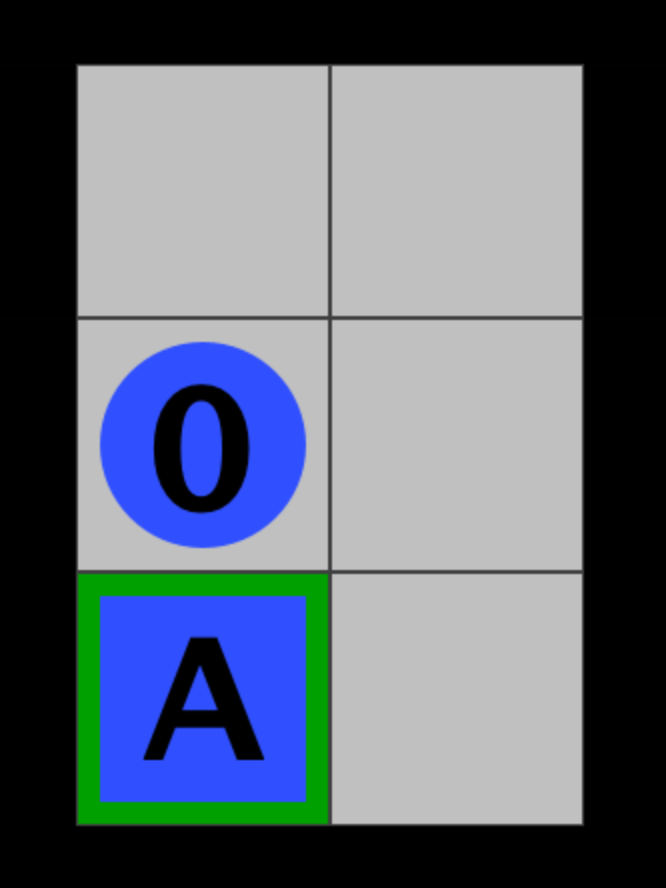
\includegraphics[width=2cm]{simple0_4} 
  \end{center}
  \caption{Solution to the level \texttt{SAsimple0.lvl}.}\label{figu:simple_solution}
\end{figure}


A \emph{solution} to a level is any sequence of joint actions that when executed in the initial state will lead to a goal state. As earlier mentioned, a goal state is any state in which every goal cell has an object of the correct type occupying it. Figure~\ref{figu:simple_level} shows a simple level, and Figure~\ref{figu:simple_solution} shows a solution to it. The solution is the action sequence \texttt{Move(S)}, \texttt{Pull(N,W)}, \texttt{Push(S,S)}.




\section{Client-server communication}\label{sect:env}


To simulate the hospital domain, use the \mavis\ server \texttt{server.jar}. The server loads a level and tracks the actual state of the world, and agents interact with the environment by communicating with the server through a client. The client communicates with the server through the standard streams \emph{stdin}, \emph{stdout}, and \emph{stderr}. Clients can thus be implemented in any programming language that can read from and write to these streams.

\begin{table}
\begin{center}
\scalebox{0.8}{
%\centering 
\setlength{\tabcolsep}{1cm} 
\begin{tabular}{lcl} 
\textsc{Server} &    & \textsc{Client}\\ \\
& 1 & \texttt{ExampleClient}\\
\texttt{\#domain} & 2 & \\
\texttt{hospital} & 3 & \\
\texttt{\#levelname} & 4 & \\
\texttt{SAExample} & 5 & \\
\texttt{\#colors} & 6 & \\
\texttt{blue: 0, A} & 7 & \\
\texttt{\#initial} & 8 & \\
\texttt{+++++} & 9 & \\
\texttt{+0A +} & 10 & \\
\texttt{+++++} & 11 & \\
\texttt{\#goal} & 12 & \\
\texttt{+++++} & 13 & \\
\texttt{+0 A+} & 14 & \\
\texttt{+++++} & 15 & \\
\texttt{\#end} & 16 & \\
& 17 & \texttt{Move(E)}\\
\texttt{false} & 18 & \\
& 19 & \texttt{Push(E,E)}\\
\texttt{true} & 20 & \\
& 21 & \texttt{Move(W)}\\
\texttt{true} & 22 & \\
\end{tabular}
}
\end{center}
\caption{Example of interaction between server and client.}
\label{tbl1:protocol_example}
\end{table}
The server and client use a text-based protocol to communicate over the streams. Table~\ref{tbl1:protocol_example} provides an example. The left and right columns show what the server and client send, respectively. The protocol text is ASCII encoded, and proceeds as follows: 
\begin{enumerate}
\item[1.] The client sends its name to the server, terminated by a newline (CRLF or LF). This is the name of the client that will be shown in the GUI of the environment simulation.
\item[2.] The server sends the contents of the level file to the client, exactly as it occurs byte-for-byte (with the addition of a final CRLF or LF if the level file is not properly terminated by a newline).
\item[3.] The client sends the server either a joint action (specified above) or a comment (which is any string starting with a hashtag symbol (\texttt{\#})). The line is terminated by a newline.
\item[4.] If the client's message was a comment, then the server prints this message to its own \emph{stdout}.
\item[5.] If the client's message was a joint action, then the server simulates the action and sends back a line of the form
\[
   \texttt{<success0>|<success1>|...|<success9>}
\]
where each \texttt{successN} is either \texttt{true} or \texttt{false} indicating whether that agent's action succeeded of failed (and where failure can either be due to inapplicability or conflicts).
\item[6.] Steps 3-5 are repeated until the client shuts down, or the server terminates the client. After the client shuts down or is terminated, the server will write a brief summary of the result to its own \emph{stdout}.
\end{enumerate}

The client receives the messages from the server on its \emph{stdin}, and sends its own messages to the server on its \emph{stdout}. Anything the client writes on its \emph{stderr} is directly redirected to whatever the server's own \emph{stderr} is connected to (typically the terminal). Thus \emph{stderr} can for instance be used for debugging purposes by writing to it during search; for example, a client may print its generated states and their heuristic values to \emph{stderr}. Table \ref{tbl1:protocol_example} illustrates a complete interaction between a server and client. The given exchange will lead to the level being solved. For details on different modes and options for the server, run the server with the \texttt{-h} argument:
\begin{verbatim}
    java -jar server.jar -h
\end{verbatim}

\end{document}
